\sectionnn{Introduction}

EnginPasTangible est un moteur graphique reposant sur le principe de Ray Marching. Un moteur graphique a pour but de fournir des rendus (images) d'une scène 3D.\par

Le Ray Marching est un système de 3D similaire au Ray Tracing, mais beaucoup moins fréquemment utilisé. Ce système possède certains avantages par rapport au Ray Tracing. 
Il permet par exemple une implémentation peu coûteuse de fractales ou autres figures se reproduisant à l'identique. \\
Le Ray Marching repose sur la projection pas à pas (\emph{Marching}) de rayons depuis une caméra vers la scène.


\begin{figure}[h]
    \centering
    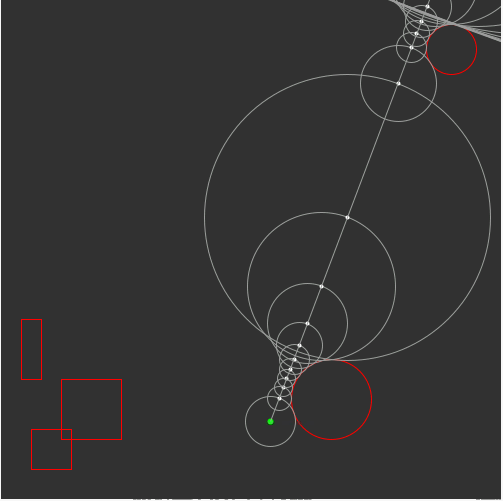
\includegraphics[width=8cm]{images/marching.png}
    \caption{Illustration 2D de la marche point par point d'un rayon (plus de détails dans \ref{subsec:projection} \nameref{subsec:projection})}
    \label{fig:my_label}
\end{figure}

Après plusieurs essais sur différentes bibliothèques de code, nous avons choisi d'utiliser le framework\footnote[1]{Infrastructure logicielle : bibliothèque de code générique} open source GLFW. Celui-ci permet l'implémentation de OpenGL Shading Language (GLSL), un langage de shading. Les langages de shading permettent une implémentation rapide des vecteurs et matrices ainsi que leurs opérations associées.\par
GLFW étant fait pour le langage C, il permet une portabilité du code sur de nombreuses plateformes telles que Windows, macOS et Linux (X11 et Wayland).\\ \par

Nos principales attentes du projet moteur graphique étaient d'apprendre à utiliser un langage de shading, et de créer un programme suffisamment performant pour obtenir des résultats en temps réel. \\
Un autre objectif était de pouvoir se déplacer de façon fluide dans la scène 3D avec des commandes intuitives.